%%%%%%%%%%%%%%%%%%%%%%%%%%%%%%%%%%%%%%%%%
% Programming/Coding Assignment
% LaTeX Template
%
% This template has been downloaded from:
% http://www.latextemplates.com
%
% Original author:
% Ted Pavlic (http://www.tedpavlic.com)
%
% Note:
% The \lipsum[#] commands throughout this template generate dummy text
% to fill the template out. These commands should all be removed when 
% writing assignment content.
%
% This template uses a Perl script as an example snippet of code, most other
% languages are also usable. Configure them in the "CODE INCLUSION 
% CONFIGURATION" section.
%
%%%%%%%%%%%%%%%%%%%%%%%%%%%%%%%%%%%%%%%%%

%----------------------------------------------------------------------------------------
% PACKAGES AND OTHER DOCUMENT CONFIGURATIONS
%----------------------------------------------------------------------------------------

\documentclass{article}

\usepackage{fancyhdr} % Required for custom headers
\usepackage{lastpage} % Required to determine the last page for the footer
\usepackage{extramarks} % Required for headers and footers
\usepackage[usenames,dvipsnames]{color} % Required for custom colors
\usepackage{graphicx} % Required to insert images
\usepackage{listings} % Required for insertion of code
\usepackage{courier} % Required for the courier font
\usepackage{lipsum} % Used for inserting dummy 'Lorem ipsum' text into the template

% Margins
\topmargin=-0.45in
\evensidemargin=0in
\oddsidemargin=0in
\textwidth=6.5in
\textheight=9.0in
\headsep=0.25in

\linespread{1.1} % Line spacing

% Set up the header and footer
\pagestyle{fancy}
\lhead{\hmwkAuthorName} % Top left header
\chead{\hmwkClass\ (\hmwkClassInstructor\ \hmwkClassTime): \hmwkTitle} % Top center head
\rhead{\firstxmark} % Top right header
\lfoot{} % Bottom left footer
\cfoot{} % Bottom center footer
\rfoot{Page\ \thepage\ of\ \protect\pageref{LastPage}} % Bottom right footer
\renewcommand\headrulewidth{0.4pt} % Size of the header rule
\renewcommand\footrulewidth{0.4pt} % Size of the footer rule

\setlength\parindent{0pt} % Removes all indentation from paragraphs

%----------------------------------------------------------------------------------------
% CODE INCLUSION CONFIGURATION
%----------------------------------------------------------------------------------------

\definecolor{MyDarkGreen}{rgb}{0.0,0.4,0.0} % This is the color used for comments
\lstloadlanguages{Perl} % Load Perl syntax for listings, for a list of other languages supported see: ftp://ftp.tex.ac.uk/tex-archive/macros/latex/contrib/listings/listings.pdf
\lstset{language=Perl, % Use Perl in this example
        frame=single, % Single frame around code
        basicstyle=\small\ttfamily, % Use small true type font
        keywordstyle=[1]\color{Blue}\bf, % Perl functions bold and blue
        keywordstyle=[2]\color{Purple}, % Perl function arguments purple
        keywordstyle=[3]\color{Blue}\underbar, % Custom functions underlined and blue
        identifierstyle=, % Nothing special about identifiers                                         
        commentstyle=\usefont{T1}{pcr}{m}{sl}\color{MyDarkGreen}\small, % Comments small dark green courier font
        stringstyle=\color{Purple}, % Strings are purple
        showstringspaces=false, % Don't put marks in string spaces
        tabsize=5, % 5 spaces per tab
        %
        % Put standard Perl functions not included in the default language here
        morekeywords={rand},
        %
        % Put Perl function parameters here
        morekeywords=[2]{on, off, interp},
        %
        % Put user defined functions here
        morekeywords=[3]{test},
        %
        morecomment=[l][\color{Blue}]{...}, % Line continuation (...) like blue comment
        numbers=left, % Line numbers on left
        firstnumber=1, % Line numbers start with line 1
        numberstyle=\tiny\color{Blue}, % Line numbers are blue and small
        stepnumber=5 % Line numbers go in steps of 5
}

% Creates a new command to include a perl script, the first parameter is the filename of the script (without .pl), the second parameter is the caption
\newcommand{\perlscript}[2]{
\begin{itemize}
\item[]\lstinputlisting[caption=#2,label=#1]{#1.pl}
\end{itemize}
}

%----------------------------------------------------------------------------------------
% DOCUMENT STRUCTURE COMMANDS
% Skip this unless you know what you're doing
%----------------------------------------------------------------------------------------

% Header and footer for when a page split occurs within a problem environment
\newcommand{\enterProblemHeader}[1]{
\nobreak\extramarks{#1}{#1 continued on next page\ldots}\nobreak
\nobreak\extramarks{#1 (continued)}{#1 continued on next page\ldots}\nobreak
}

% Header and footer for when a page split occurs between problem environments
\newcommand{\exitProblemHeader}[1]{
\nobreak\extramarks{#1 (continued)}{#1 continued on next page\ldots}\nobreak
\nobreak\extramarks{#1}{}\nobreak
}

\setcounter{secnumdepth}{0} % Removes default section numbers
\newcounter{homeworkProblemCounter} % Creates a counter to keep track of the number of problems

\newcommand{\homeworkProblemName}{}
\newenvironment{homeworkProblem}[1][Question \arabic{homeworkProblemCounter}]{ % Makes a new environment called homeworkProblem which takes 1 argument (custom name) but the default is "Problem #"
\stepcounter{homeworkProblemCounter} % Increase counter for number of problems
\renewcommand{\homeworkProblemName}{#1} % Assign \homeworkProblemName the name of the problem
\section{\homeworkProblemName} % Make a section in the document with the custom problem count
\enterProblemHeader{\homeworkProblemName} % Header and footer within the environment
}{
\exitProblemHeader{\homeworkProblemName} % Header and footer after the environment
}

\newcommand{\problemAnswer}[1]{ % Defines the problem answer command with the content as the only argument
\noindent\framebox[\columnwidth][c]{\begin{minipage}{0.98\columnwidth}#1\end{minipage}} % Makes the box around the problem answer and puts the content inside
}

\newcommand{\homeworkSectionName}{}
\newenvironment{homeworkSection}[1]{ % New environment for sections within homework problems, takes 1 argument - the name of the section
\renewcommand{\homeworkSectionName}{#1} % Assign \homeworkSectionName to the name of the section from the environment argument
\subsection{\homeworkSectionName} % Make a subsection with the custom name of the subsection
\enterProblemHeader{\homeworkProblemName\ [\homeworkSectionName]} % Header and footer within the environment
}{
\enterProblemHeader{\homeworkProblemName} % Header and footer after the environment
}

%----------------------------------------------------------------------------------------
% NAME AND CLASS SECTION
%----------------------------------------------------------------------------------------

\newcommand{\hmwkTitle}{Assignment\ \#2} % Assignment title
\newcommand{\hmwkDueDate}{Thursday,\ March\ 5,\ 2015} % Due date
\newcommand{\hmwkClass}{Introduction to Digital Libraries\ CS-751} % Course/class
\newcommand{\hmwkClassTime}{4:20pm} % Class/lecture time
\newcommand{\hmwkClassInstructor}{Michael L. Nelson} % Teacher/lecturer
\newcommand{\hmwkAuthorName}{Avinash Gosavi} % Your name

%----------------------------------------------------------------------------------------
% TITLE PAGE
%----------------------------------------------------------------------------------------

\title{
\vspace{2in}
\textmd{\textbf{\hmwkClass:\ \hmwkTitle}}\\
\normalsize\vspace{0.1in}\small{Due\ on\ \hmwkDueDate}\\
\vspace{0.1in}\large{\textit{\hmwkClassInstructor\ \hmwkClassTime}}
\vspace{3in}
}

\author{\textbf{\hmwkAuthorName}}
\date{} % Insert date here if you want it to appear below your name

%----------------------------------------------------------------------------------------

\begin{document}

\maketitle

%----------------------------------------------------------------------------------------
% TABLE OF CONTENTS
%----------------------------------------------------------------------------------------

%\setcounter{tocdepth}{1} % Uncomment this line if you don't want subsections listed in the ToC

\newpage
\tableofcontents
\newpage

%----------------------------------------------------------------------------------------
% PROBLEM 1
%----------------------------------------------------------------------------------------

% To have just one problem per page, simply put a \clearpage after each problem

\begin{homeworkProblem}
Choose 100 URIs from A1\\
Generate WARC files of those URIs using:\\
wget\\
WARCreate\\
Heritrix (stand-alone or via WAIL)\\
webrecorder.io\\
Describe the resulting WARC files: quantitatively compare \& contrast the results of the WARC files of the same URI as generated by different tools
choose interesting examples\\
Demonstrate playback of 2-3 WARCs in the (Wayback Machine (via WAIL or stand-alone) or pywb) and (webrecorder.io)
% https://github.com/iipc/openwayback 
% https://github.com/ikreymer/pywb
% Listing \ref{homework_example} shows a Perl script.

% \perlscript{homework_example}{Sample Perl Script With Highlighting}
\end{homeworkProblem}

\section{Answer}

WARC can be created using following four tools wget, WARCreate, Heritrix and webrecorder.io.\\

wget was the simplest to implement. It was just one line of code.\\

WARCreate is a chrome plugin to create a warc of current file. It was not creating WARC’s for certain urls and from what I observed it was not doing it for pages that have deep links like imdb.\\

Heritrix warc was done using WAIL. Setting up wail took a lot of time. Wail configuration was also not straightforward. It was taking time to create WARC for certain urls as they had many sub pages. So later on a configuration was added to heritrix to restrict by time size and documents in heritrix job config file.\\

Webrecorder.io is an online tool for creating and replaying WARC file. It was simple to use.
In Webrecorder.io was pretty useful in replaying WARC files created from all four methods. \\


Figures 1 to 15 are screenshot for replay of warc generated by using Heritrix, WARCreate, webrecorder.io and wget in the same order. Also after every example I am adding description and comparison for warc files. Urls for the three url are as below
1) https://twitter.com/rachidblog1/status/564533520916561923
2) http://willbrooks.deviantart.com/art/Doctor-Who-Titles-GIF-491765997
3) http://www.f1technical.net/features/19903\\

Figure 16, 17 \& 18 are graphs comparing sizes for warc files created by different tools.\\

The sizes of warc files do depend on the method that we use to generate the warc file. Wget has the least size for all four URI. Heritrix would always have bigger size because it always crawls into sub-pages for a URI. The size of WARC also depends on url we are trying to call. If it has more media and deep pages it will be of bigger size. \\


\clearpage


%----------------------------------------------------------------------------------------
% PROBLEM 2
%----------------------------------------------------------------------------------------

\begin{homeworkProblem}

Ingest the 100 URIs from their resulting WARC files into a SOLR instance
% see the code + tutorial at: https://github.com/ukwa/webarchive-discovery 
Demonstrate several functioning queries on the files (a full front-end is not required)
describe the configuration choices you made in setting up SOLR and processing the documents

\end{homeworkProblem}

\section{Answer}


Solr has configurations to specify things like what we can index from warc files and what shouldn’t be indexed. We can specify if images are to be extracted or not.\\

For processing documents in solr I executed following command.

\begin{verbatim}
java -jar warc-indexer-2.0.1-20150116.110435-2-jar-with-dependencies.jar \
  -s http://localhost:8080/discovery -t \
  /Users/avinashgosavi/projects/cs851-s15/assignment2/wget-combined-warc
\end{verbatim}

For running queries I kept the default configuration given in webarchive-discovery.\\

Figure 19 shows a query to return urls for domain twitter. This would give links from twitter.\\
Figure 20 shows a query to return urls that org as public suffix. This would give me all org domain urls.

%----------------------------------------------------------------------------------------

\clearpage


\section{Figures}

\begin{center}
\begin{figure}[ht]
    \centering
    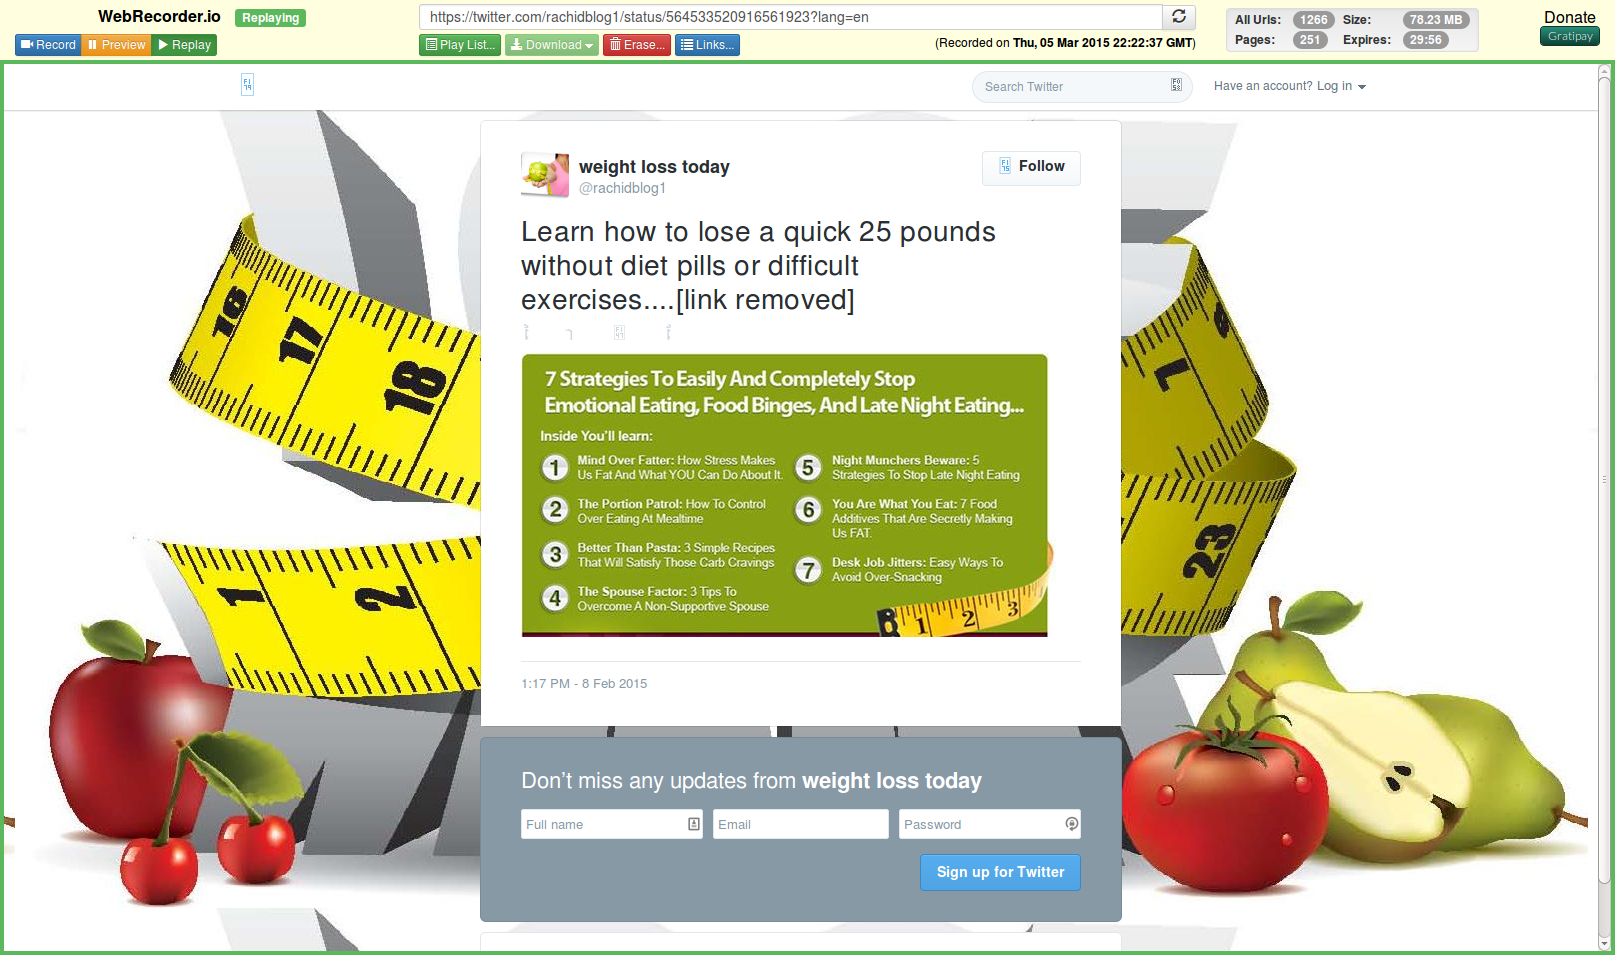
\includegraphics[width=0.475\textwidth,natwidth=700,natheight=700]{ex1-heritrix.png}
    \caption{Heritrix}
    \label{fig:url1_heritrix}
\end{figure}
\begin{figure}[ht]
    \centering
    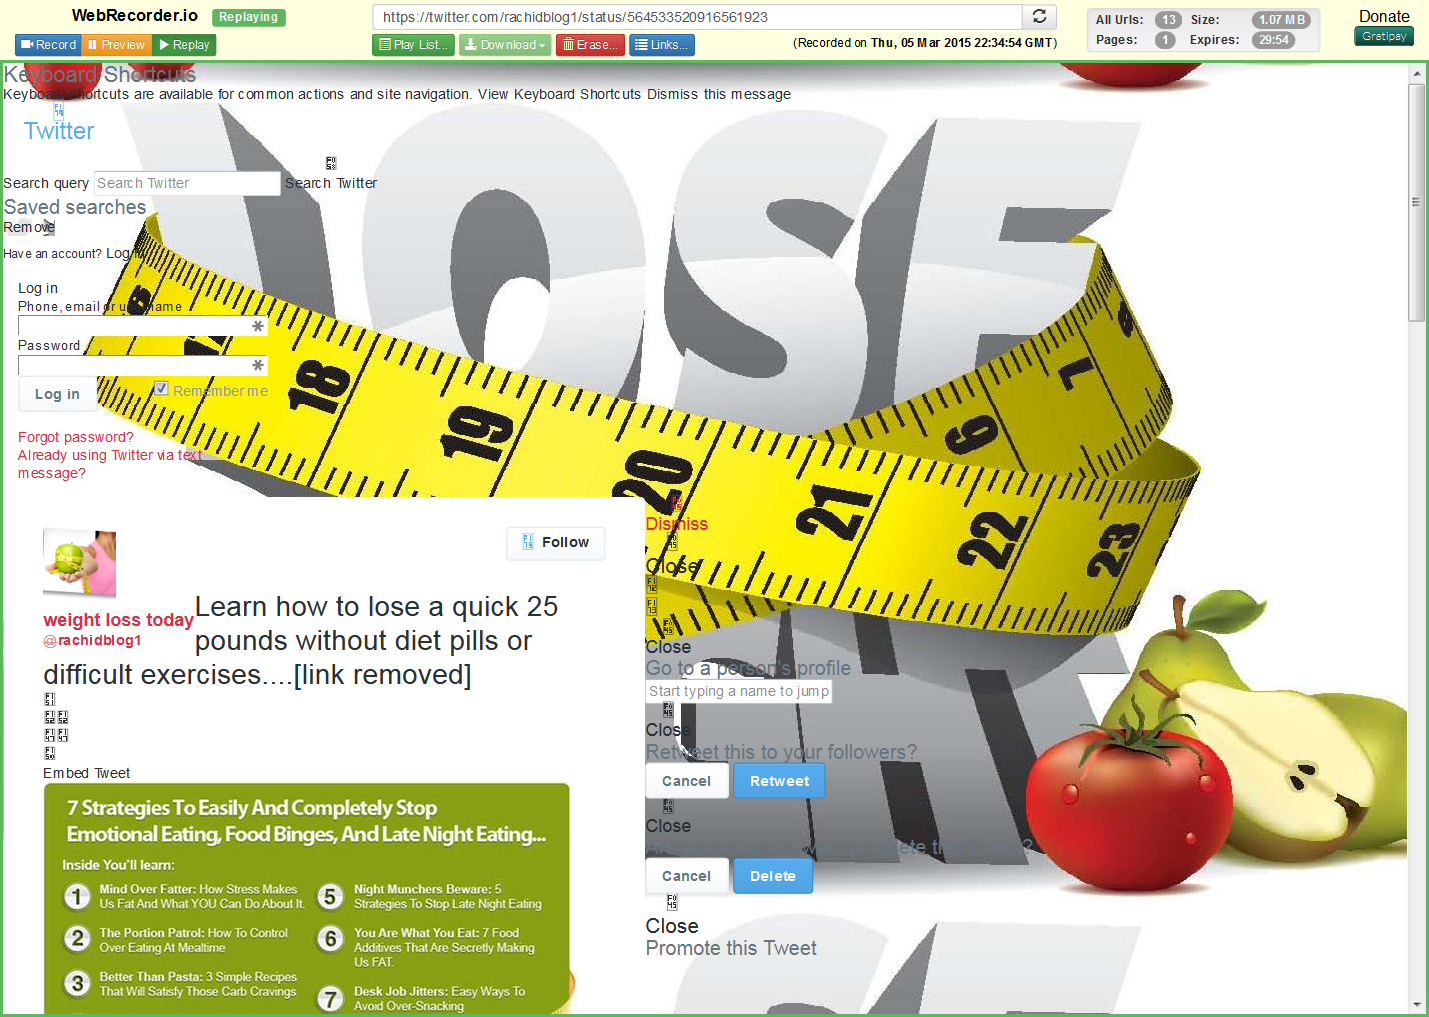
\includegraphics[width=0.475\textwidth,natwidth=700,natheight=700]{ex1-warcreate.png}
    \caption{WARCreate}
    \label{fig:url1_war_create}
\end{figure}
\begin{figure}[ht]
    \centering
    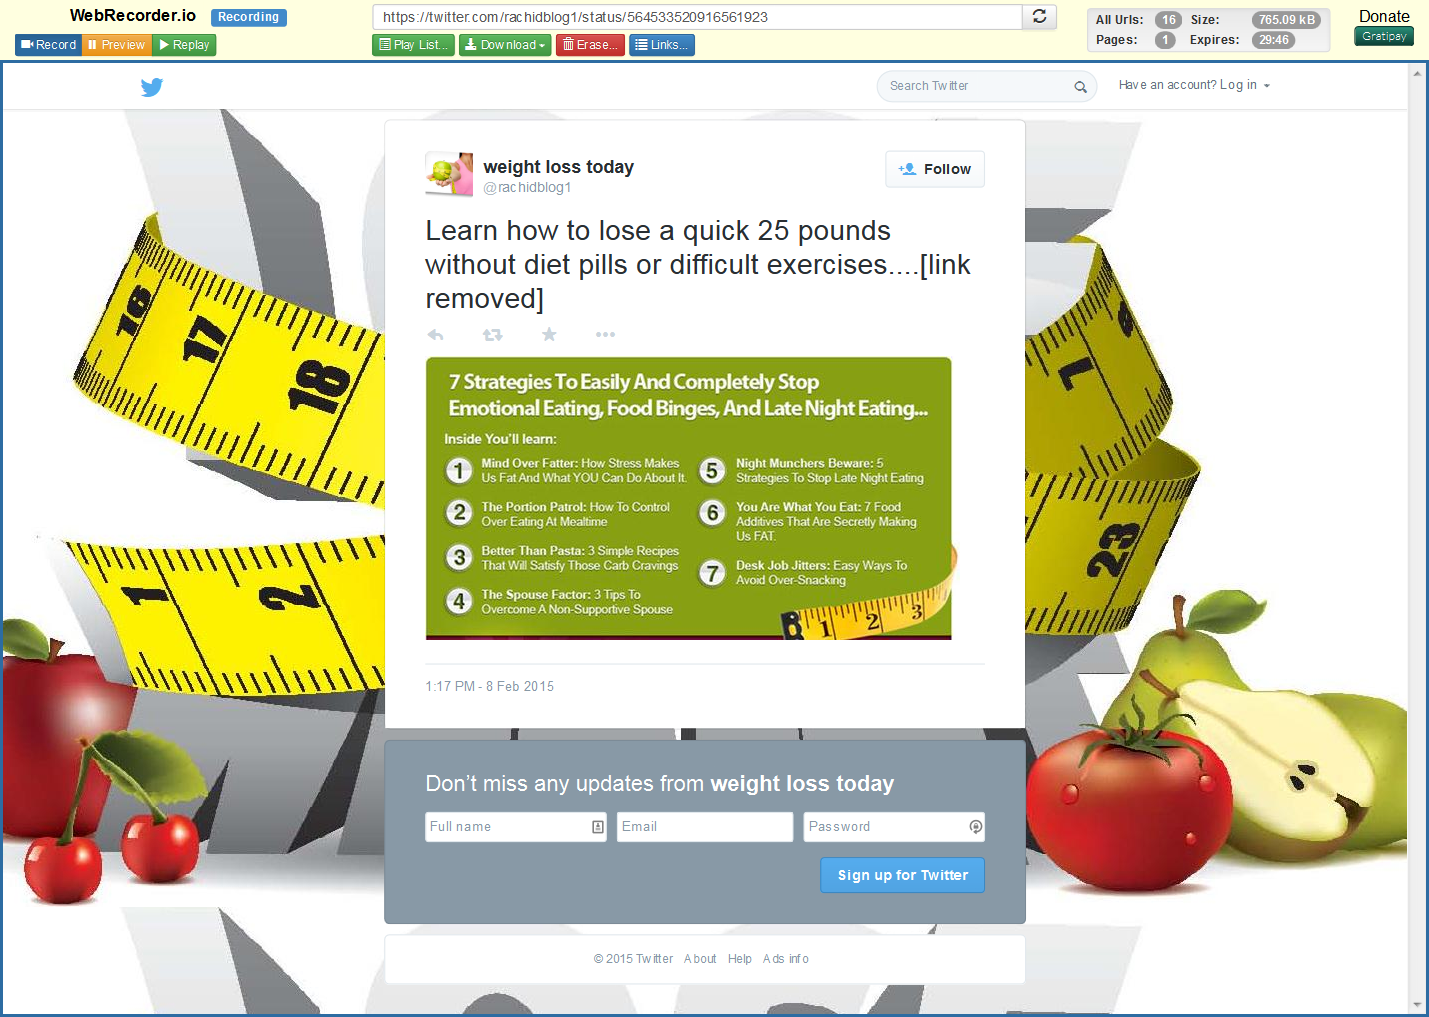
\includegraphics[width=0.475\textwidth,natwidth=700,natheight=700]{ex1-webrecorder.png}
    \caption{Webrecorder.io}
    \label{fig:url1_webrecorder}
\end{figure}
\begin{figure}[ht]
    \centering
    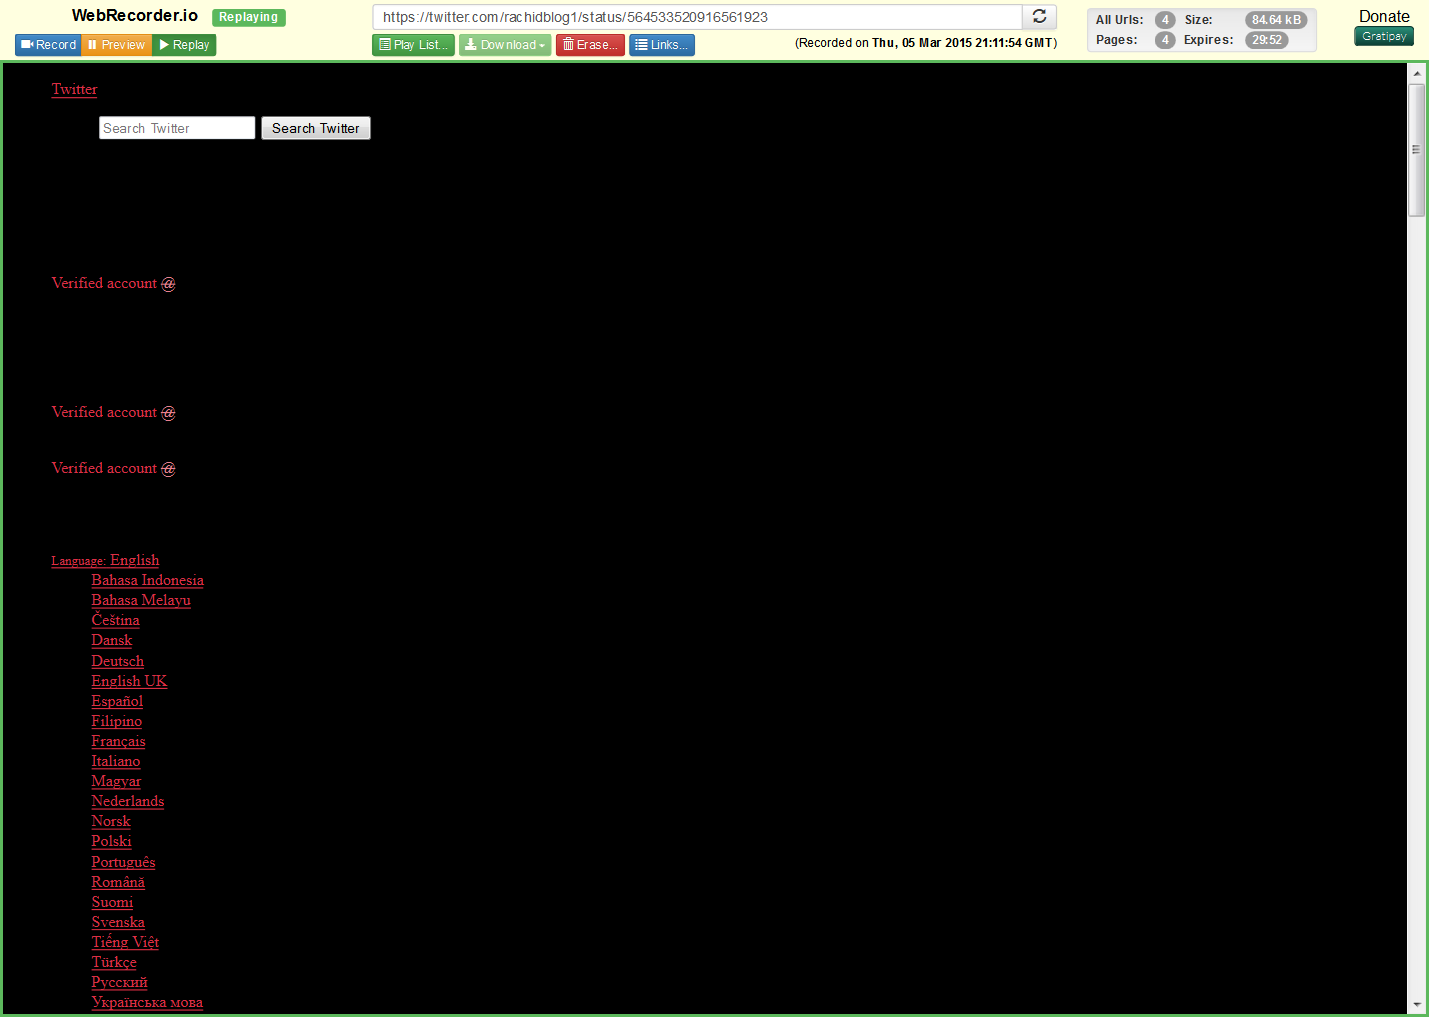
\includegraphics[width=0.475\textwidth,natwidth=700,natheight=700]{ex1-wget.png}
    \caption{wget}
    \label{fig:url1_wget}
\end{figure}
\begin{figure}[ht]
    \centering
    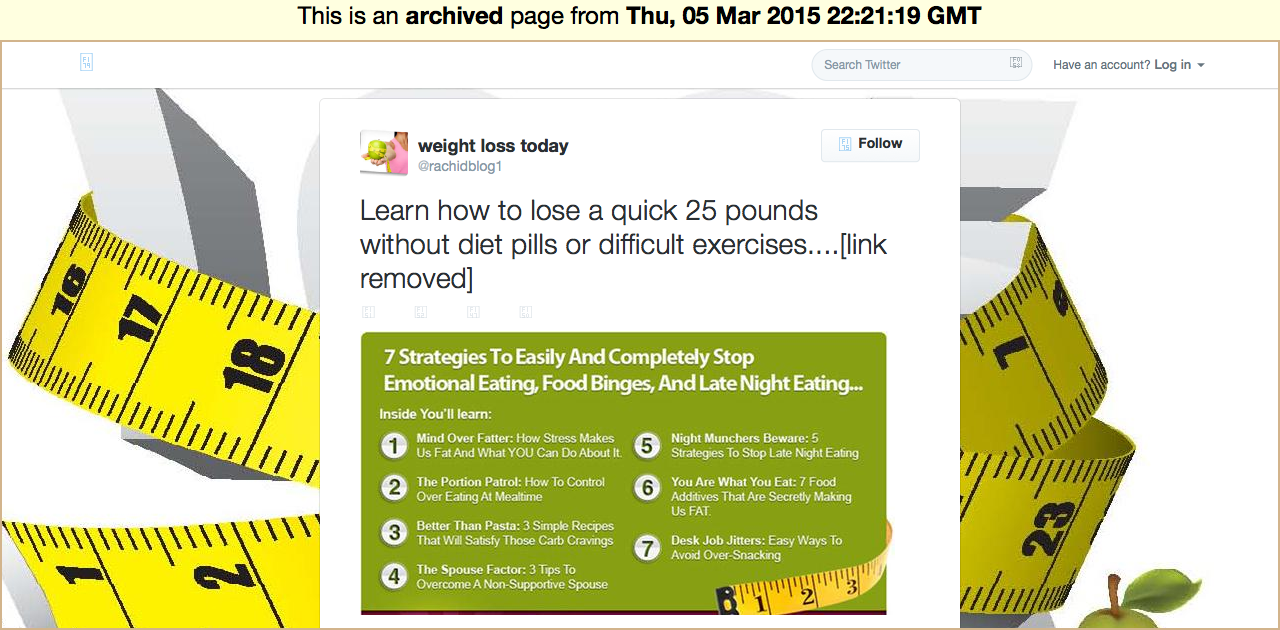
\includegraphics[width=0.475\textwidth,natwidth=700,natheight=700]{ex1-heritrix-pywb.png}
    \caption{Heritrix - pywb}
    \label{fig:url1_heritrix_pywb}
\end{figure}
\end{center}

\clearpage

\begin{center}
\begin{figure}[ht]
    \centering
    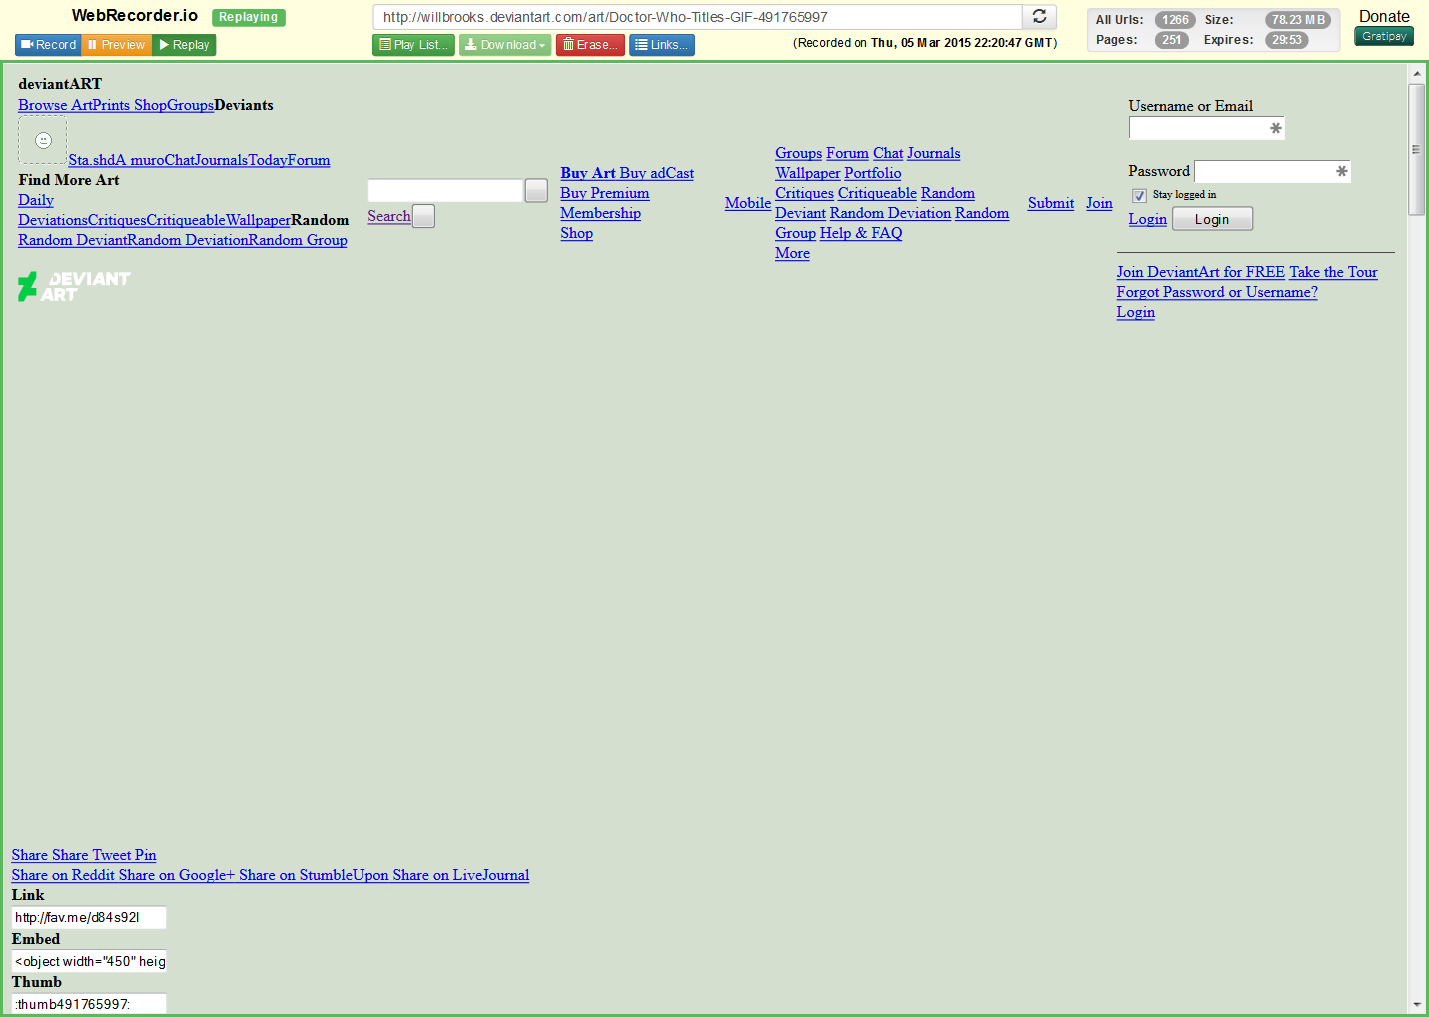
\includegraphics[width=0.475\textwidth,natwidth=700,natheight=700]{ex2-heritrix.png}
    \caption{Heritrix}
    \label{fig:url2_heritrix}
\end{figure}
\begin{figure}[ht]
    \centering
    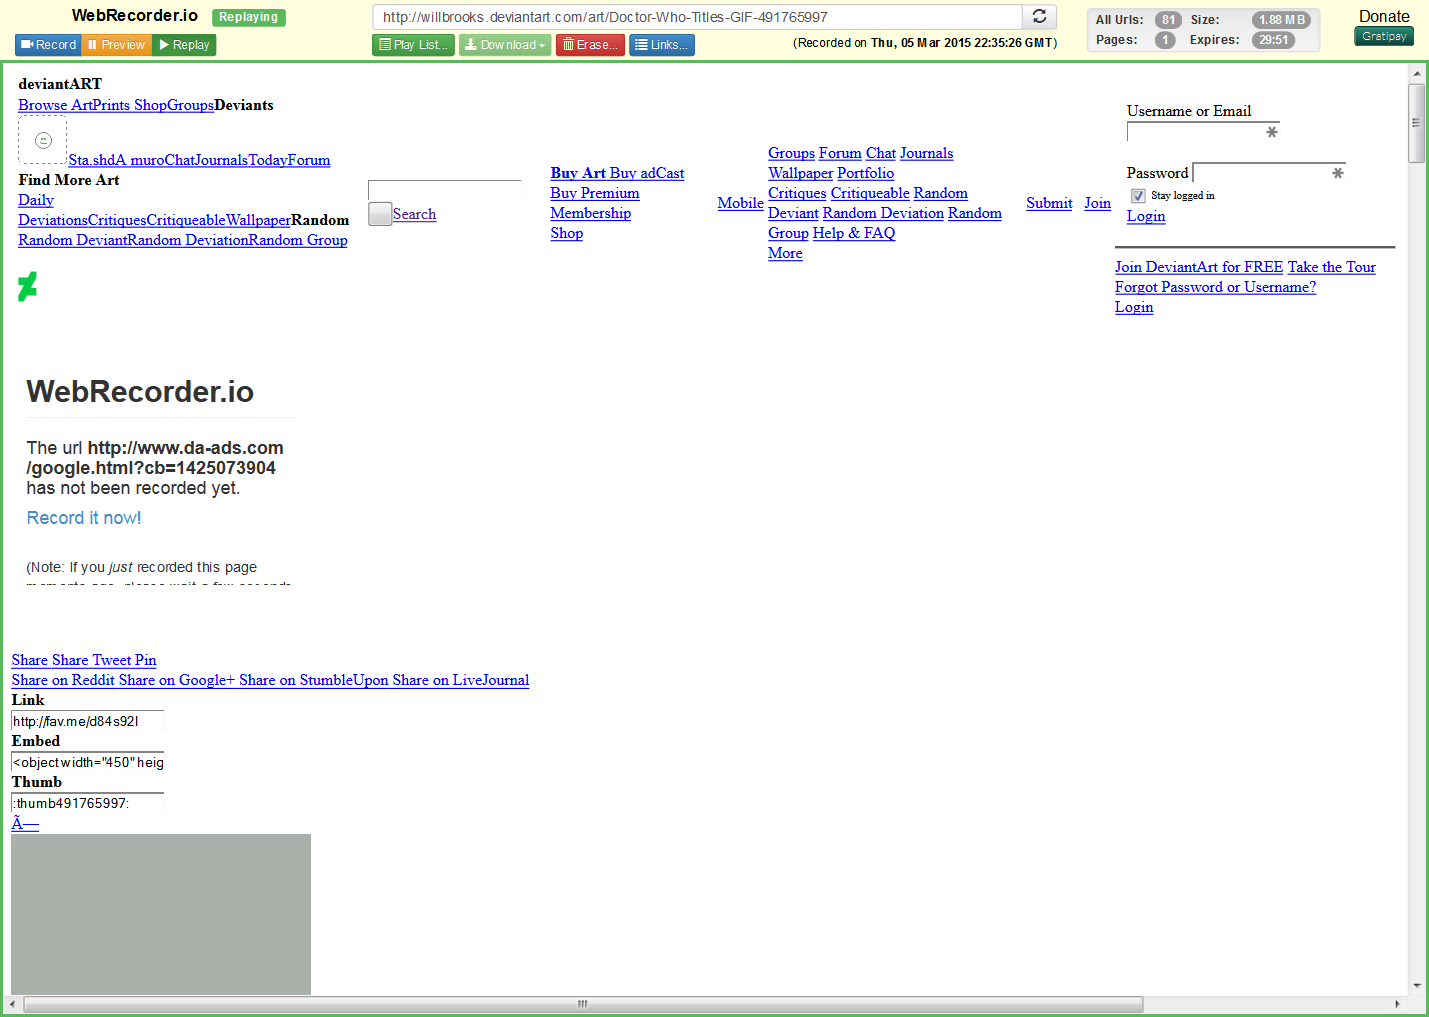
\includegraphics[width=0.475\textwidth,natwidth=700,natheight=700]{ex2-warcreate.png}
    \caption{WARCreate}
    \label{fig:url2_war_create}
\end{figure}
\begin{figure}[ht]
    \centering
    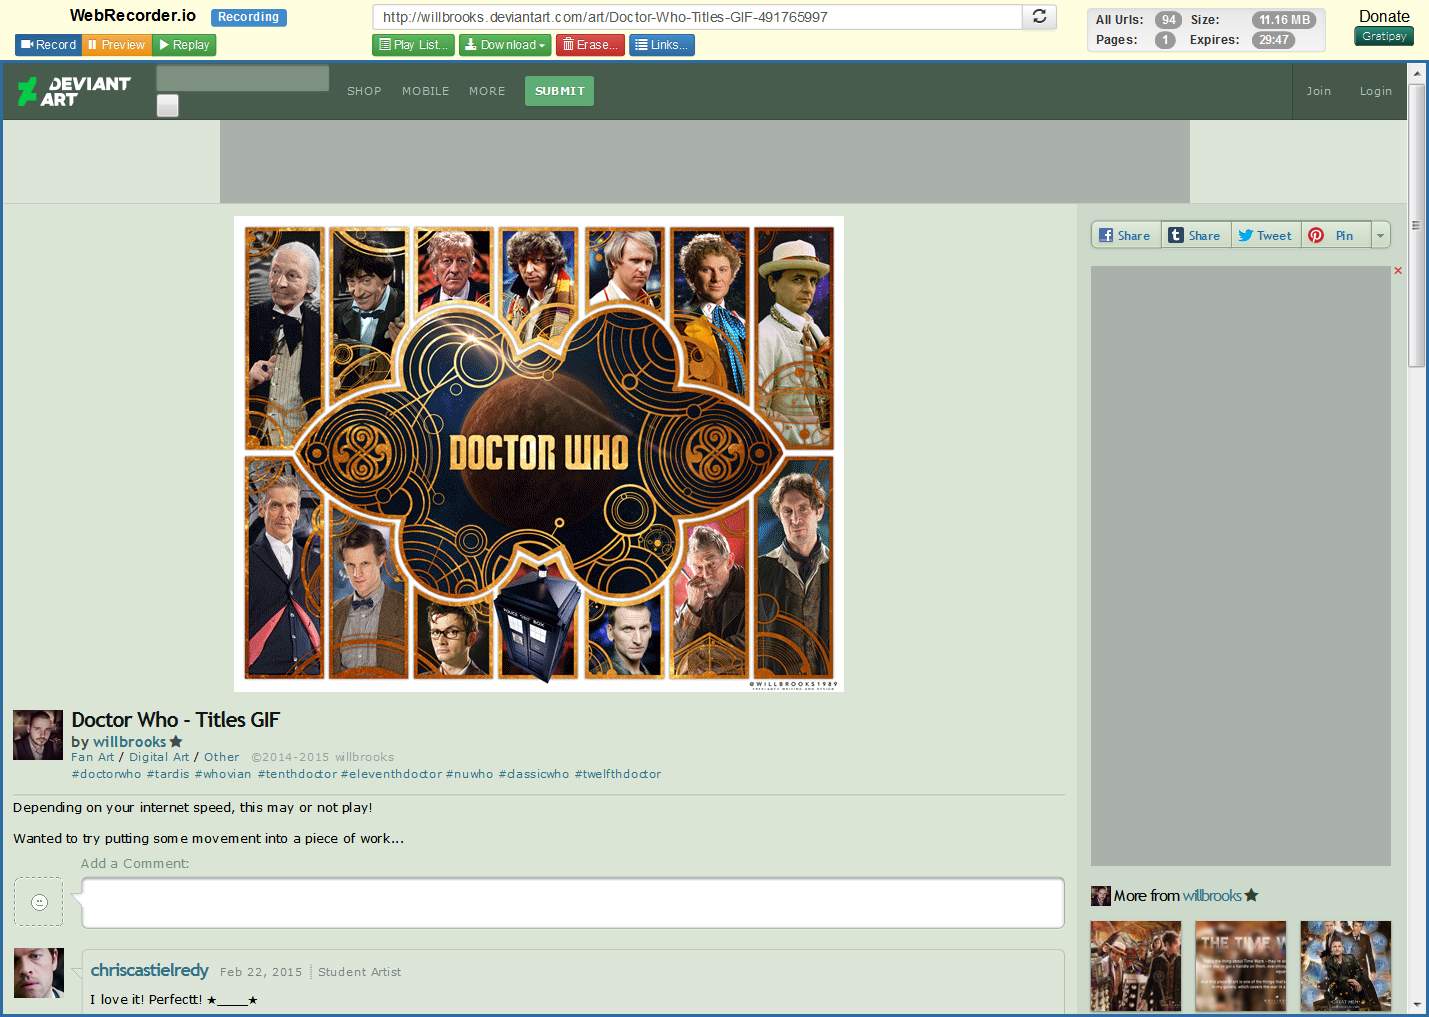
\includegraphics[width=0.475\textwidth,natwidth=700,natheight=700]{ex2-webrecorder.png}
    \caption{Webrecorder.io}
    \label{fig:url2_webrecorder}
\end{figure}
\begin{figure}[ht]
    \centering
    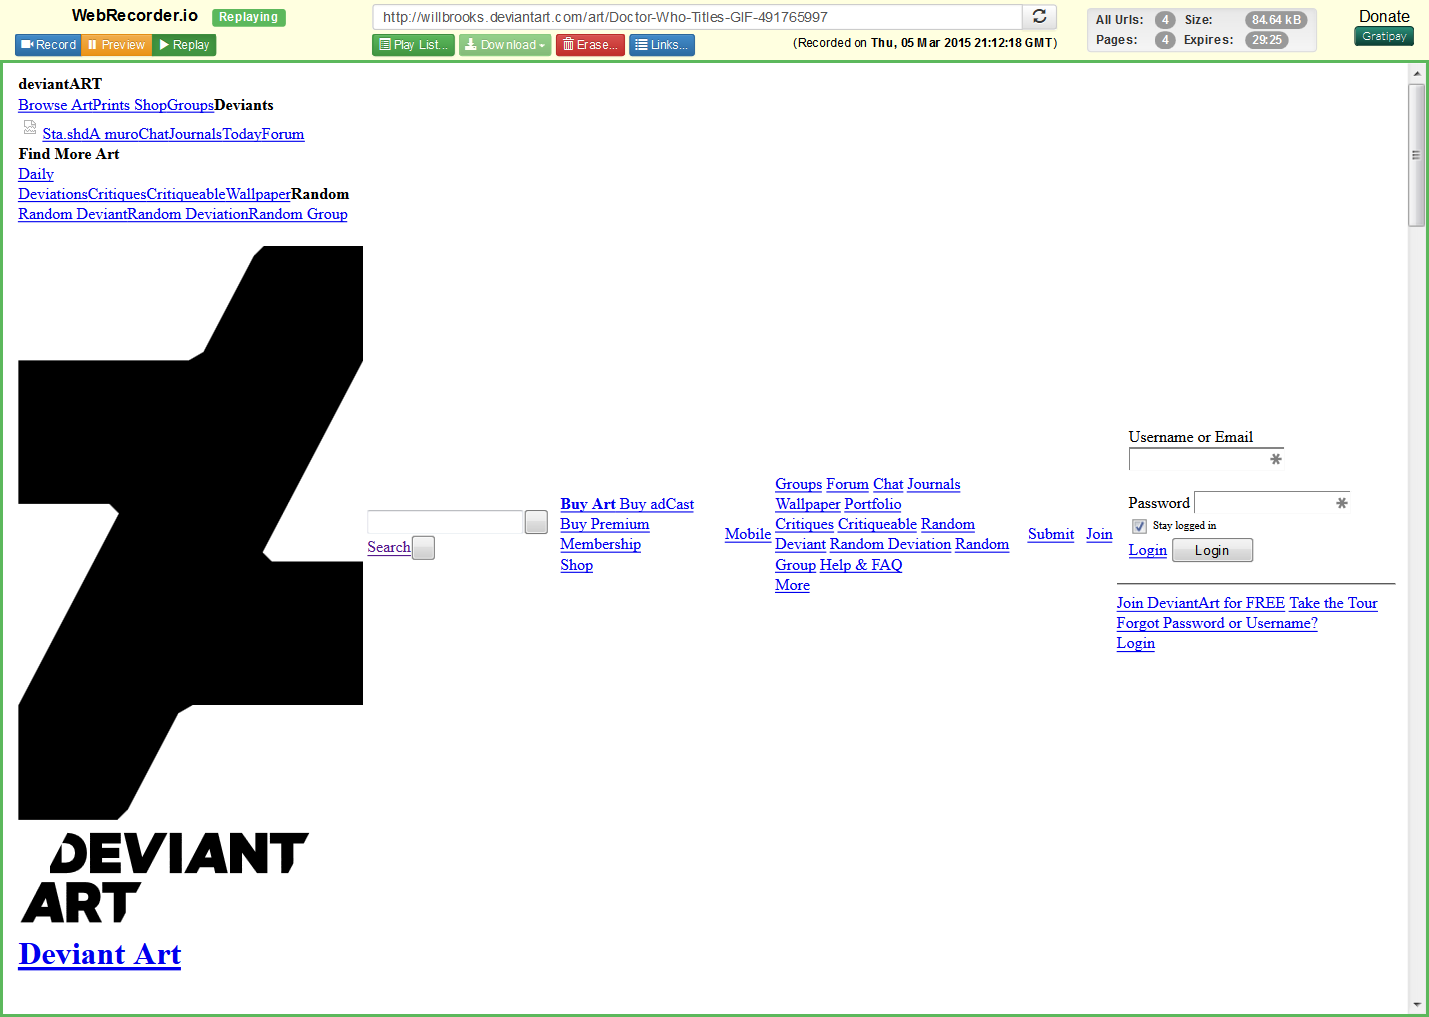
\includegraphics[width=0.475\textwidth,natwidth=700,natheight=700]{ex2-wget.png}
    \caption{wget}
    \label{fig:url2_wget}
\end{figure}
\begin{figure}[ht]
    \centering
    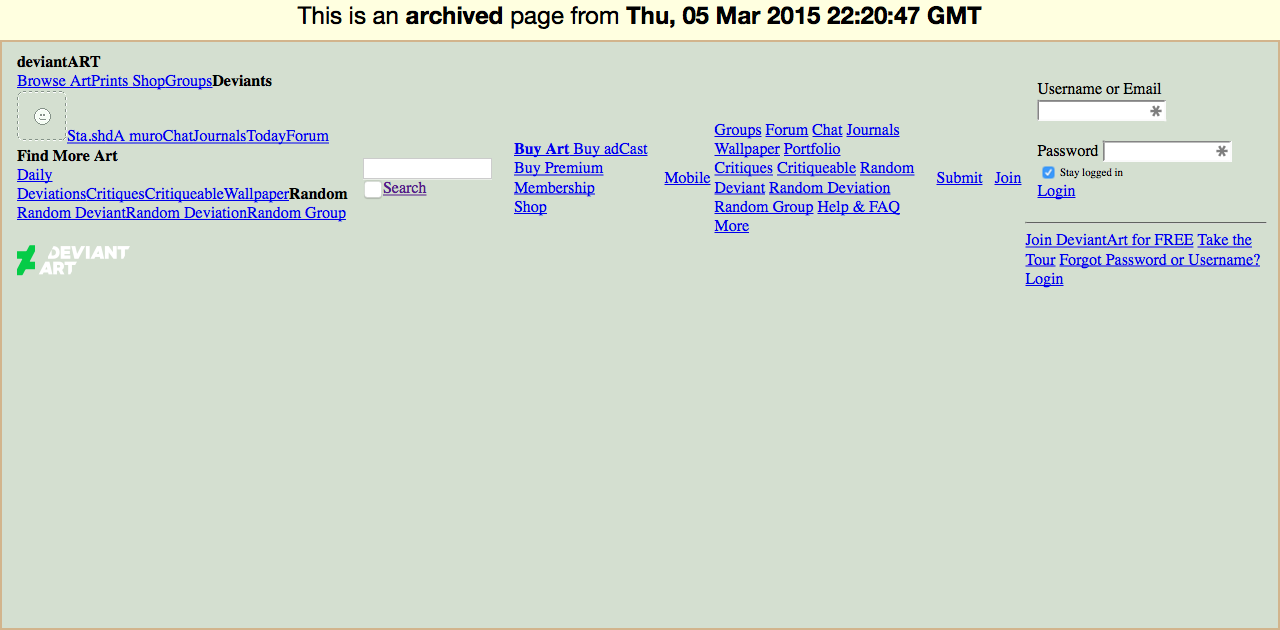
\includegraphics[width=0.475\textwidth,natwidth=700,natheight=700]{ex2-heritrix-pywb.png}
    \caption{Heritrix - pywb}
    \label{fig:url2_heritrix_pywb}
\end{figure}
\end{center}

\clearpage

\begin{center}
\begin{figure}[ht]
    \centering
    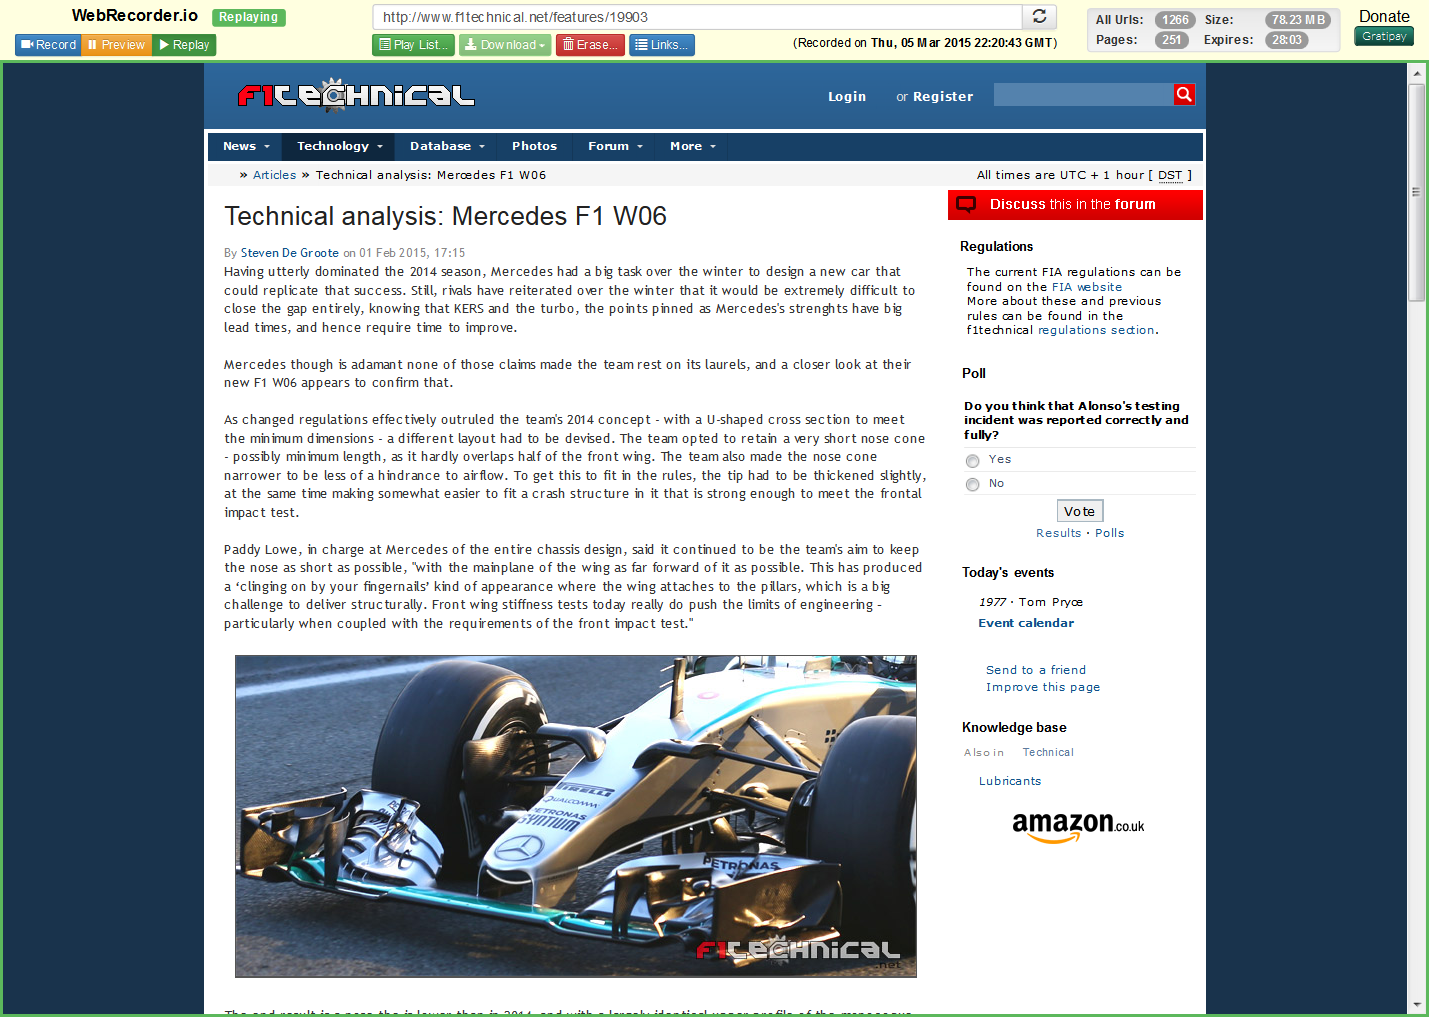
\includegraphics[width=0.475\textwidth,natwidth=700,natheight=700]{ex3-heritrix.png}
    \caption{Heritrix}
    \label{fig:url3_heritrix}
\end{figure}
\begin{figure}[ht]
    \centering
    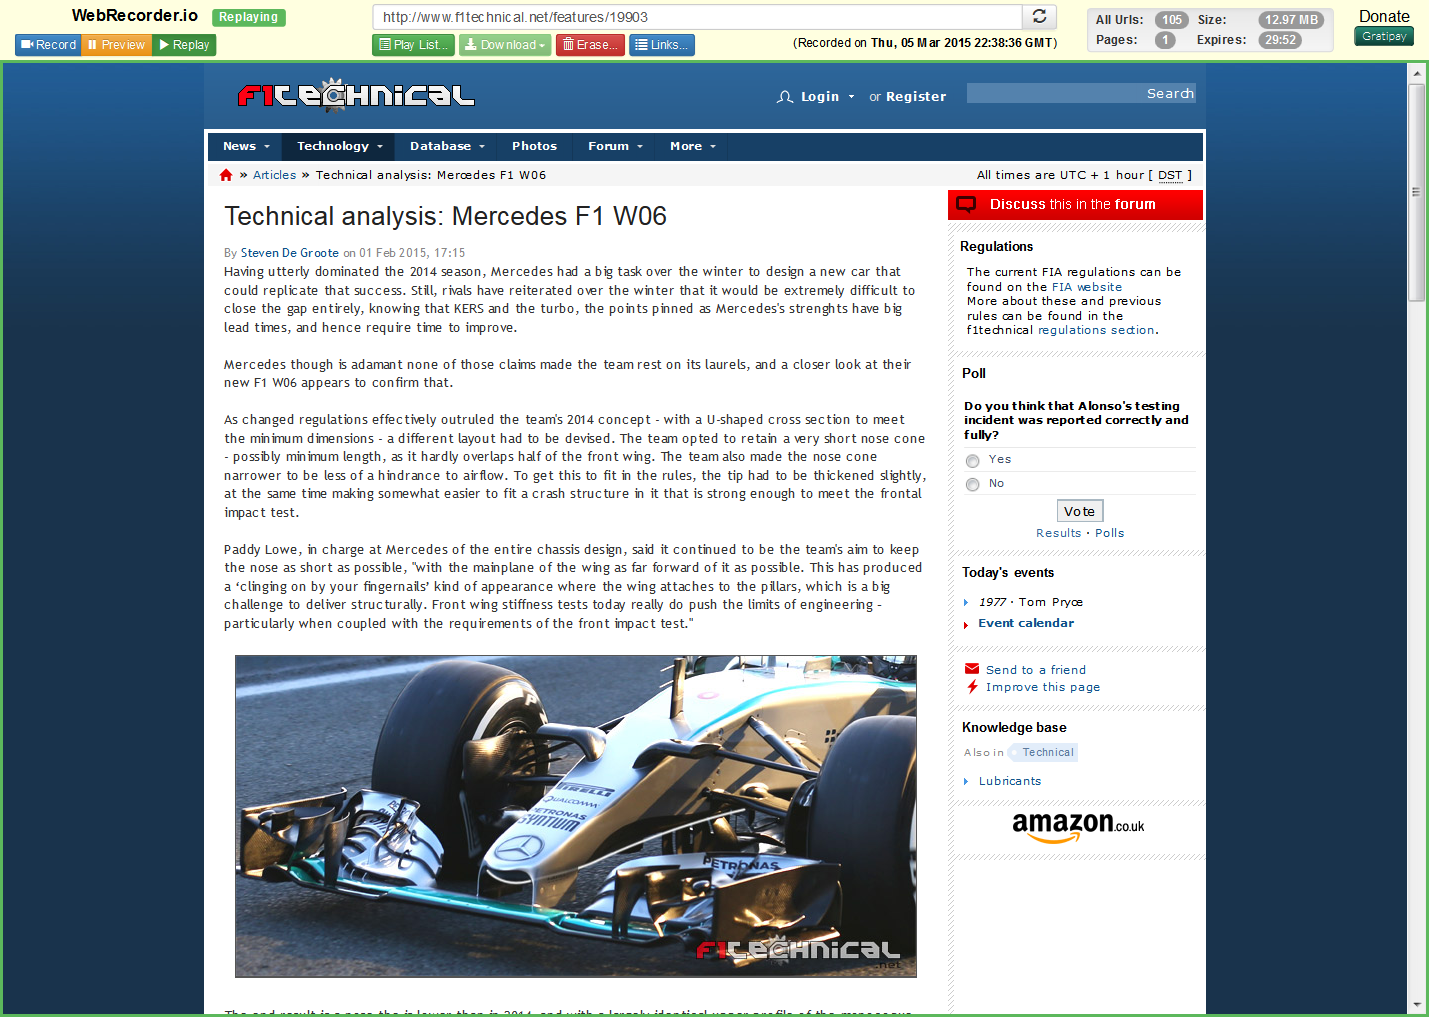
\includegraphics[width=0.475\textwidth,natwidth=700,natheight=700]{ex3-warcreate.png}
    \caption{WARCreate}
    \label{fig:url3_war_create}
\end{figure}
\begin{figure}[ht]
    \centering
    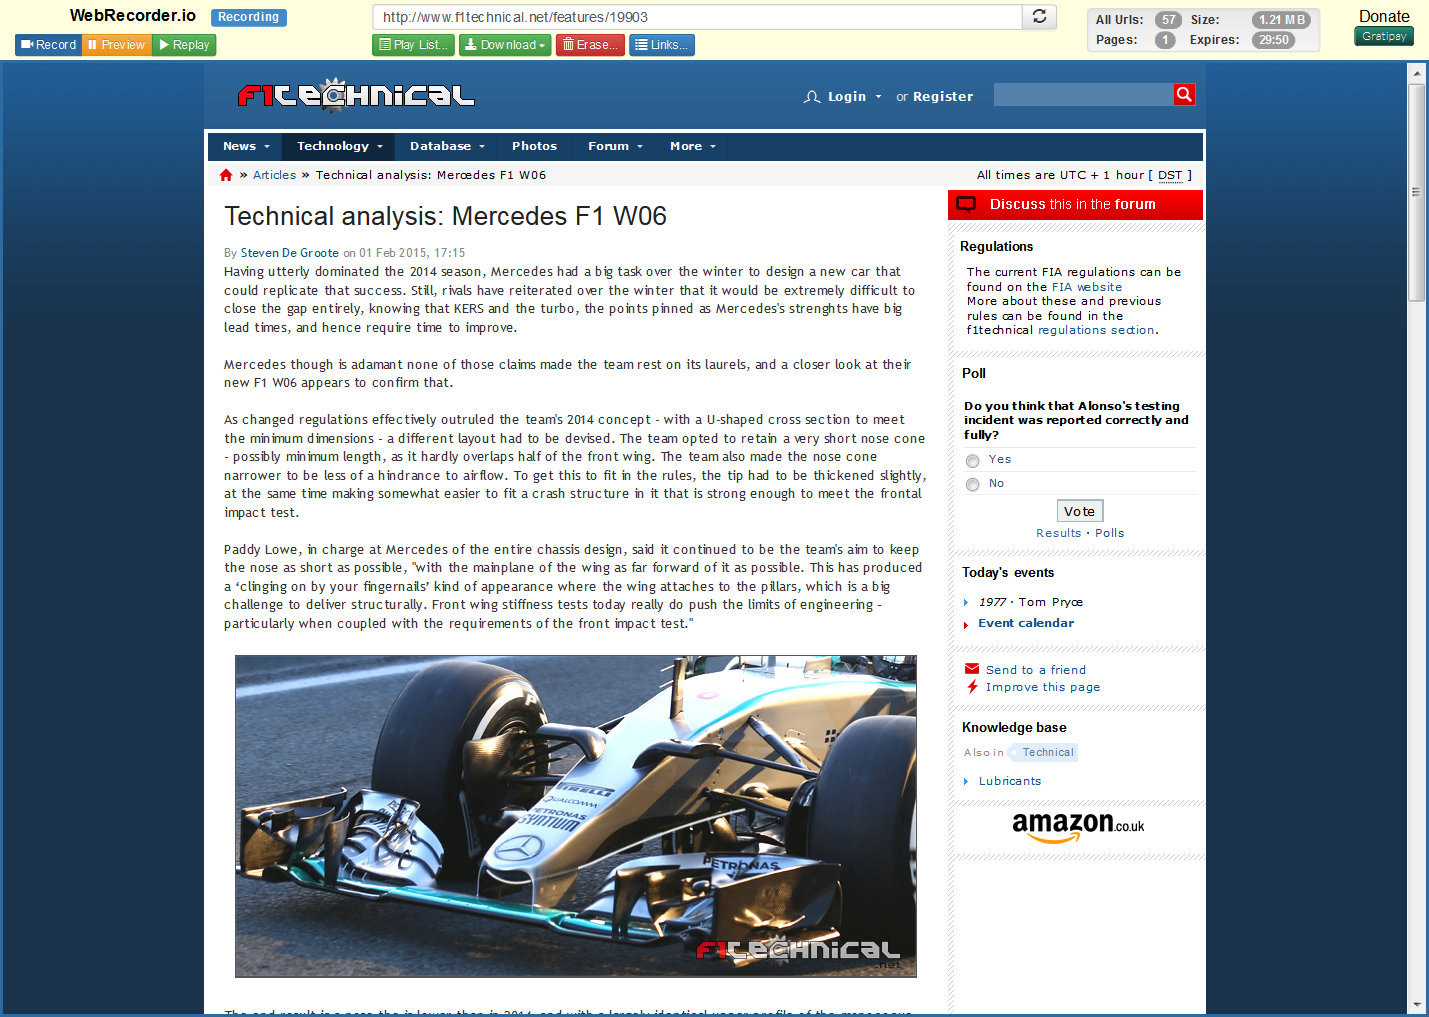
\includegraphics[width=0.475\textwidth,natwidth=700,natheight=700]{ex3-webrecorder.png}
    \caption{Webrecorder.io}
    \label{fig:url3_webrecorder}
\end{figure}
\begin{figure}[ht]
    \centering
    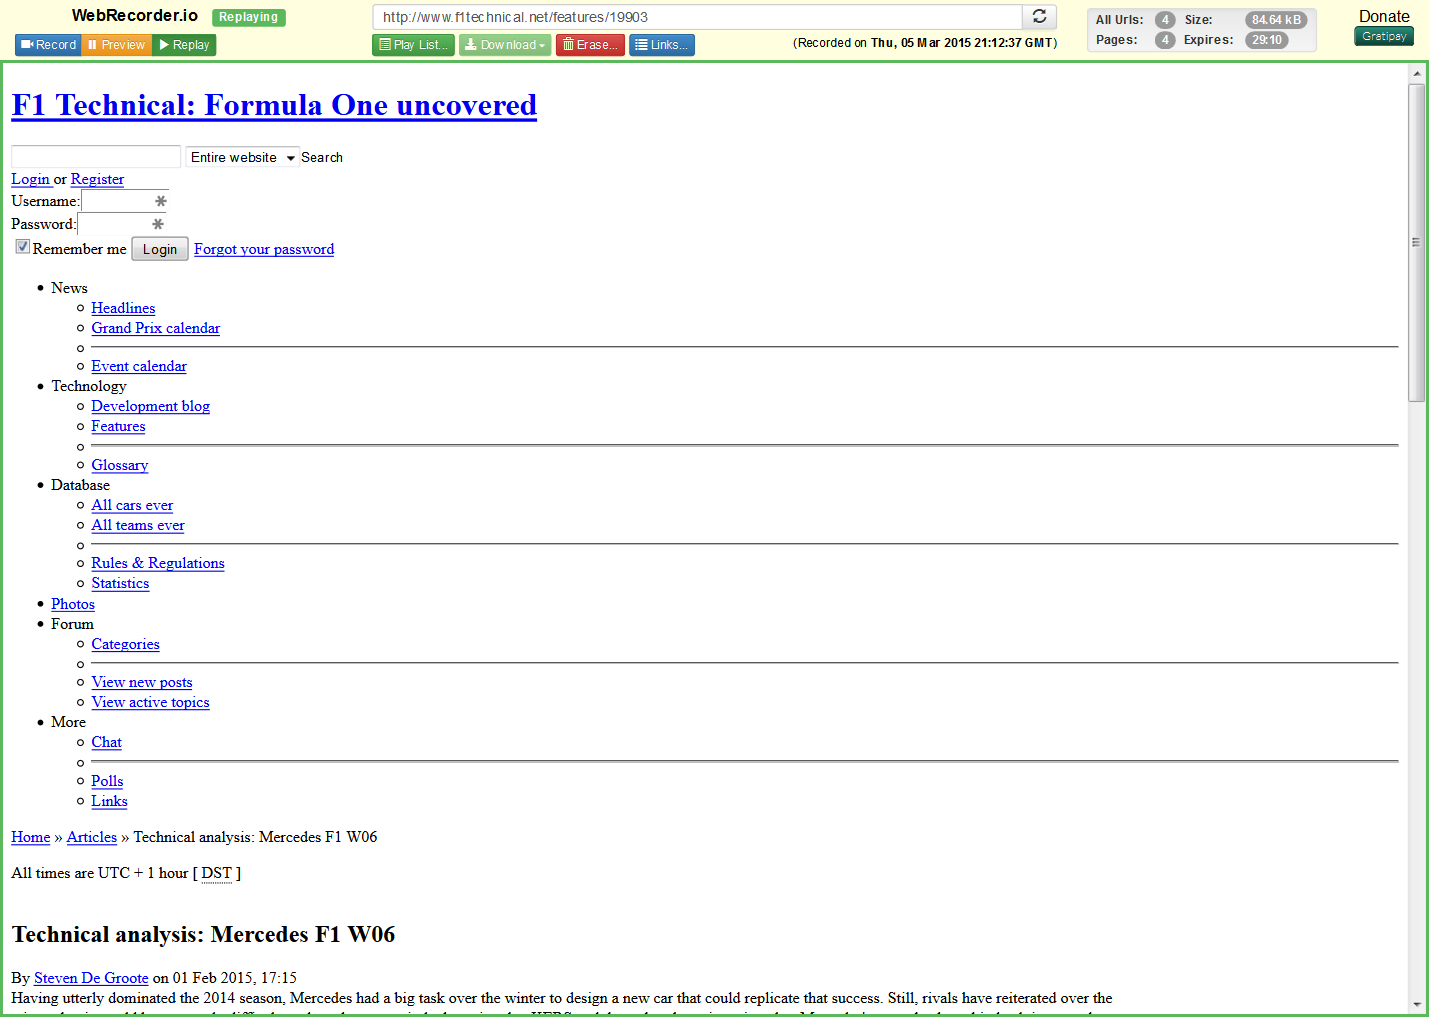
\includegraphics[width=0.475\textwidth,natwidth=700,natheight=700]{ex3-wget.png}
    \caption{wget}
    \label{fig:url3_wget}
\end{figure}
\begin{figure}[ht]
    \centering
    
\includegraphics[width=0.475\textwidth,natwidth=700,natheight=700]{ex3-heritrix-pywb.png}
    \caption{Heritrix - pywb}
    \label{fig:url3_heritrix_pywb}
\end{figure}
\end{center}

\clearpage

\begin{center}
\begin{figure}[ht]
    \centering
    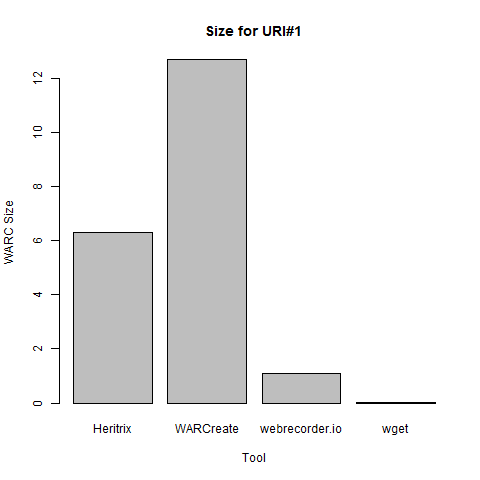
\includegraphics[width=0.475\textwidth,natwidth=700,natheight=700]{graph1.png}
    \caption{Graph 1}
    \label{fig:graph1}
\end{figure}
\begin{figure}[ht]
    \centering
    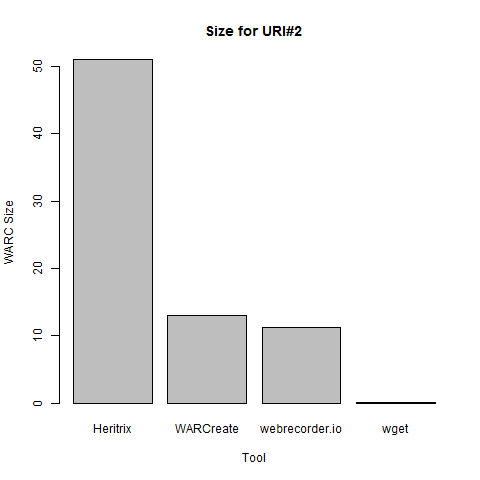
\includegraphics[width=0.475\textwidth,natwidth=700,natheight=700]{graph2.png}
    \caption{Graph 2}
    \label{fig:graph2}
\end{figure}
\begin{figure}[ht]
    \centering
    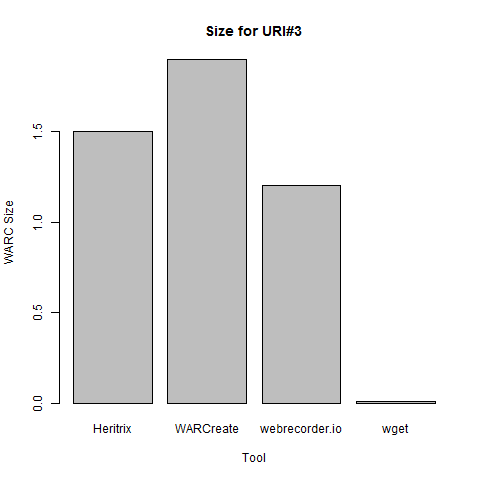
\includegraphics[width=0.475\textwidth,natwidth=700,natheight=700]{graph3.png}
    \caption{Graph 3}
    \label{fig:graph3}
\end{figure}
\end{center}

\begin{center}
\begin{figure}[ht]
    \centering
    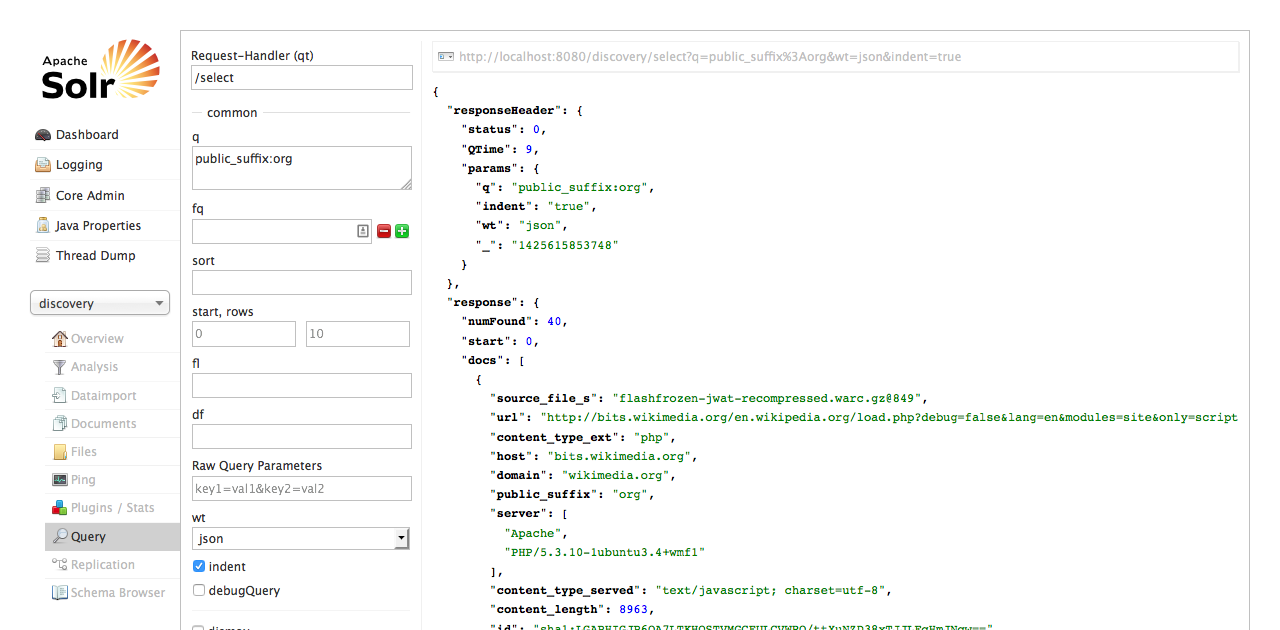
\includegraphics[width=0.475\textwidth,natwidth=700,natheight=700]{solar_public_prefix.png}
    \caption{Solr 1}
    \label{fig:solr1}
\end{figure}
\begin{figure}[ht]
    \centering
    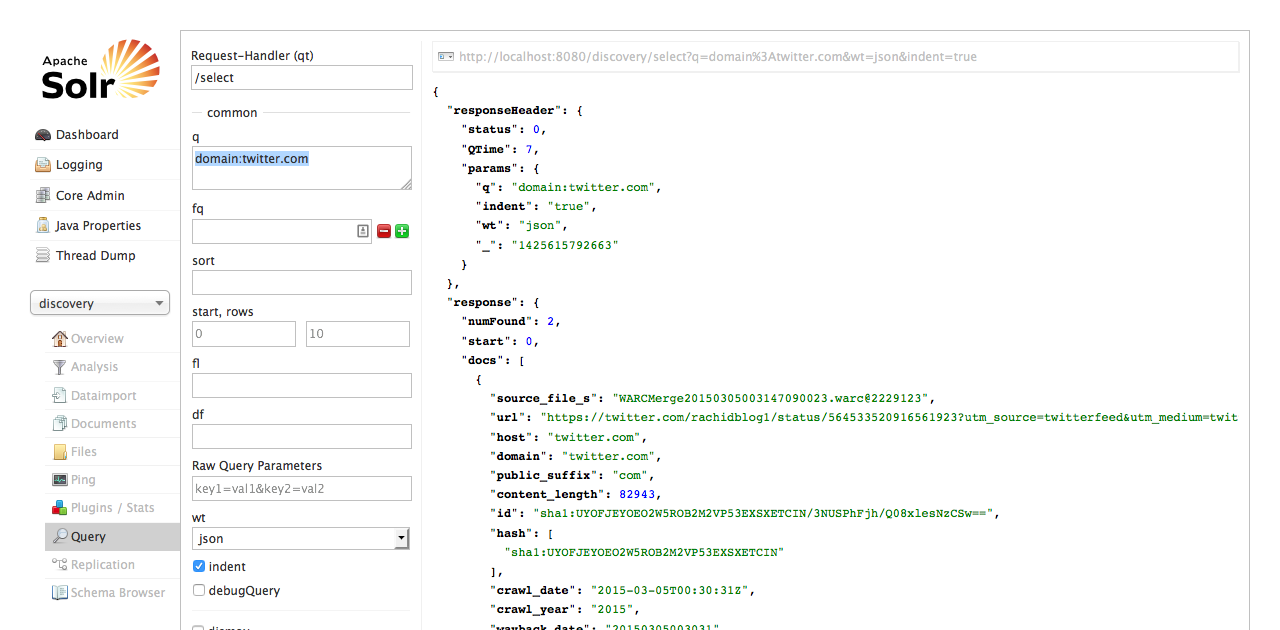
\includegraphics[width=0.475\textwidth,natwidth=700,natheight=700]{solr_domain_twitter.png}
    \caption{Solr 2}
    \label{fig:solr2}
\end{figure}
\end{center}

\clearpage

\end{document}